% !TeX encoding = UTF-8
% !TeX program = pdflatex
% !TeX spellcheck = it_IT

\documentclass[Lau, binding=0.6cm, italian]{sapthesis}

\graphicspath{assets/}

\usepackage{microtype}
\usepackage[italian]{babel}
\usepackage[utf8]{inputenx}
\usepackage{wrapfig}
\usepackage{cprotect}
\usepackage{listings}
\usepackage{float}

\renewcommand{\lstlistingname}{Snippet} % Listing -> Snippet

\definecolor{codegreen}{rgb}{0,0.6,0}
\definecolor{codeblue}{rgb}{0,0.20,1}
\definecolor{codegray}{rgb}{0.5,0.5,0.5}
\definecolor{codepurple}{rgb}{0.58,0,0.82}
\definecolor{backcolour}{rgb}{0.95,0.95,0.92}

\lstdefinestyle{JavaCustom}{
    backgroundcolor=\color{backcolour},   
    commentstyle=\color{codegreen},
    keywordstyle=\color{codeblue},
    numberstyle=\tiny\color{codegray},
    stringstyle=\color{codepurple},
    basicstyle=\ttfamily\footnotesize,
    breakatwhitespace=false,         
    breaklines=true,                 
    captionpos=b,                    
    keepspaces=true,                 
    numbers=left,                    
    numbersep=5pt,                  
    showspaces=false,                
    showstringspaces=false,
    showtabs=false,                  
    tabsize=2
}

\lstset{style=JavaCustom}

\usepackage{hyperref}
\hypersetup
{
	pdftitle={Progettazione e sviluppo di piattaforma per la gestione di risorse linguistiche},
	pdfauthor={Andrea Gasparini}
}

\usepackage{lipsum}
\usepackage{curve2e}

\title{Progettazione e sviluppo di piattaforma per la gestione di risorse linguistiche}
\author{Andrea Gasparini}
\IDnumber{1813486}
\course{Informatica}
\courseorganizer{Facoltà di Ingegneria dell'informazione, informatica e statistica}
\AcademicYear{2019/2020}
\copyyear{2020}
\advisor{Prof. Roberto Navigli}
\authoremail{gasparini.1813486@studenti.uniroma1.it}
\examdate{14 Dicembre 2020}
\examiner{Prof. Roberto Navigli}
\examiner{Prof. Emiliano Casalicchio}
\examiner{Prof. Pietro Cenciarelli}
\examiner{Prof. Luigi Cinque}
\examiner{Prof. Daniele Gorla}
\examiner{Prof. Walter Quattrociocchi}
\examiner{Prof. Adolfo Piperno}
\versiondate{\today}

\begin{document}

\frontmatter

\maketitle

\begin{abstract}
	L'oggetto del tirocinio è la progettazione e lo sviluppo di una piattaforma web
	per migliorare la gestione delle risorse linguistiche di \textbf{SapienzaNLP},
	il gruppo di ricerca del dipartimento di Informatica che si occupa di multilingual
	Natural Language Understanding.

	La relazione è divisa in 4 parti fondamentali: l'introduzione allo \textbf{scenario
	di riferimento} e alla necessità del lavoro svolto; l'\textbf{analisi dei requisiti},
	volta a migliorare la modellazione delle funzionalità della piattaforma; la
	\textbf{progettazione del sistema} e della sua architettura; i dettagli
	dello sviluppo e delle \textbf{fasi di implementazione}.
\end{abstract}

\tableofcontents

\mainmatter

% !TeX root = ../relazione.tex

\chapter{Introduzione}


\section{Le risorse linguistiche nell'NLP}
Il Natural Language Processing (NLP) è un settore dell'intelligenza artificiale
che studia i problemi legati a comprensione, analisi e generazione automatica del
linguaggio naturale (come ad esempio un testo scritto o una conversazione orale).
Il \textbf{Natural Language Understanding} (NLU) \cite{navigli2018natural} è un argomento
specifico dell'NLP che riguarda in particolare la capacità delle macchine di leggere
e comprendere il significato di un testo, e più in generale del linguaggio naturale.
È facile rendersi conto di quanto sia complesso l'obiettivo che l'NLU si pone,
per via della grande ambiguità che può avere il linguaggio umano, basti pensare
ai diversi significati che una stessa frase può assumere in base al contesto del
discorso.
Nell'affrontare questa tematica è quindi importante prendere in considerazione
la struttura sintattica e l'analisi semantica, ovvero rispettivamente la
disposizione delle parole in una frase secondo un criterio ben preciso e del
significato che sta dietro alle parole anche nel contesto della frase.

\paragraph{Cos'è una risorsa linguistica?}
Per far si che un algoritmo di NLP possa elaborare un testo basandosi su sintassi
e semantica in maniera automatica è necessario che possa "imparare" a partire
da dei dati linguistici strutturati.
Una risorsa contenente questa tipologia di dati e che ne consenta facilmente il
trattamento e l'analisi da parte di una macchina viene detta \textbf{risorsa linguistica}.
Da non confondere con i dizionari informatizzati, il cui scopo è limitato a
fornire informazioni linguistiche sul lessico di una lingua e che sono costruiti
per essere consultati solamente da un utente umano.

Inizialmente la costruzione di risorse linguistiche avveniva manualmente, come
ad esempio per WordNet e FrameNet, ma questo richiedeva un grande impegno in
termini di tempi e costi.
Solo negli ultimi anni si sono sperimentati altri approcci per la creazione
delle risorse, da quelli automatici o semi-automatici, in cui parte del lavoro
viene svolto da una macchina, a quelli collaborativi che sarebbero impensabili
senza l'ausilio di internet.

\paragraph{WordNet \cite{Miller1990}}
WordNet è una delle più importanti e storiche risorse linguistiche per l'inglese.
Il progetto, nato nel 1985 e ancora oggi molto utilizzato, si basa sull'idea
di creare un dizionario in cui la ricerca non avviene alfabeticamente ma concettualmente.
All'interno di WordNet le parole sono organizzate in gruppi di sinonimi detti
\textit{synset}, dall'inglese synonyms set, ciascuno dei quali rappresenta un
concetto lessicale.
La struttura è quella di un grafo, in cui i nodi rappresentano i synset e gli archi
le relazioni lessicali e semantico-concettuali presenti tra loro.

\paragraph{BabelNet \cite{NavigliPonzetto:12aij}}
Una delle principali risorse linguistiche pubblicate da SapienzaNLP è BabelNet,
un dizionario enciclopedico multilingue consultabile online\footnote{\url{https://babelnet.org}},
creato integrando automaticamente risorse come Wikipedia, WordNet, Wiktionary,
Wikidata e molte altre.
BabelNet è allo stesso tempo una rete semantica che collega concetti, lemmi
ed entità nominate tramite delle relazioni semantiche chiamate \textbf{Babel synset}.
Ogni Babel synset comprende diverse lingue e rappresenta uno specifico significato
raggruppando tutti i sinonimi che lo esprimono, con relative definizioni ed esempi.

Attualmente BabelNet supporta 284 lingue diverse, per un totale di 15,780,364
Babel synsets, 808,974,108 sensi, 277,036,611 relazioni semantico-lessicali.

\begin{figure}[ht]
	\centering
	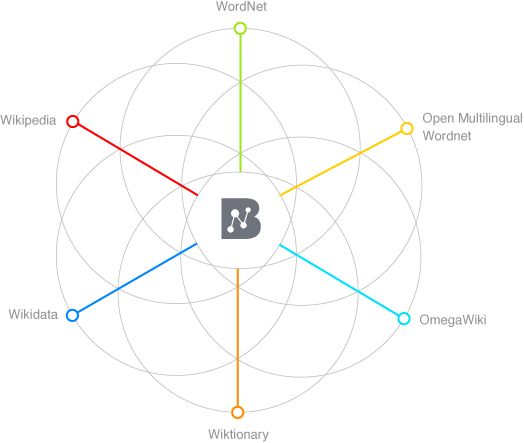
\includegraphics[width=0.75\textwidth]{assets/babelnet.png}
\end{figure}



\section{Le licenze software}
Come in generale per qualunque prodotto software, anche l'utilizzo delle risorse
pubblicate da SapienzaNLP è sempre vincolato da delle licenze d'uso, ovvero una
serie di autorizzazioni che vengono concesse all'utente per quanto riguarda l'utilizzo,
la modifica e l'eventuale ridistribuzione.

Le tipologie di licenze esistenti nell'ambito software sono molteplici e possono
variare da un utilizzo a fini commerciali, come ad esempio \textbf{OEM}
che consente l'utilizzo del software preinstallato sull'hardware che si acquista
ma vincolandolo solo ad esso, fino ad un utilizzo completamente libero, come per
\textbf{GNU General Public License} la quale permette di accedere al codice sorgente,
modificarlo e ridistribuirne delle copie -- anche a pagamento -- fintanto che questo
avvenga utilizzando la stessa licenza.
Un'esigenza molto comune è quella di avere delle licenze personalizzate ad hoc
per casi specifici, ma nel farlo è importante tenere in considerazione molteplici
aspetti e questioni giuridiche per poter distribuire tranquillamente il software. 

\paragraph{Le licenze Creative Commons (CC) \cite{cc:licenses}}
Creative Commons è un'organizzazione no-profit nata con lo scopo di semplificare
e standardizzare le modalità per ottenere una licenza personalizzata in base alla
combinazione di 4 semplici clausole:
\begin{itemize}
	\item \textbf{Attribution} (BY), che impone di dover sempre indicare l'autore	
	\item \textbf{Non Commercial} (NC), che impedisce l'utilizzo per fini commerciali
	\item \textbf{No Derivative Works} (ND), che impedisce rielaborazioni e ridistribuzioni
	\item \textbf{Share Alike} (SA), che consente di modificare e ridistribuire
	fintanto che venga utilizzata la stessa licenza
\end{itemize}
Oltre a rendere disponibile una semplice pagina web\footnote{\url{https://creativecommons.org/choose/}}
che in base alle proprie preferenze consiglia la licenza più adatta, al fine di rendere
le licenze più accessibili possibile, vengono rese disponibili in 3 diversi "livelli":
\begin{itemize}
	\item \textbf{Legal Code} che consiste nella licenza vera e propria, composta
	di termini tecnici e giuridici
	\item \textbf{Common Deed} -- anche detto "Human Readable" -- che contiene
	un breve riepilogo delle clausole presenti, chiarendo cosa è permesso e cosa no
	\item \textbf{Machine Readable} che rappresenta la licenza in un formato strutturato
	di facile interpretazione all'interno di un motore di ricerca o di un software
\end{itemize}

\begin{figure}[ht]
	\centering
	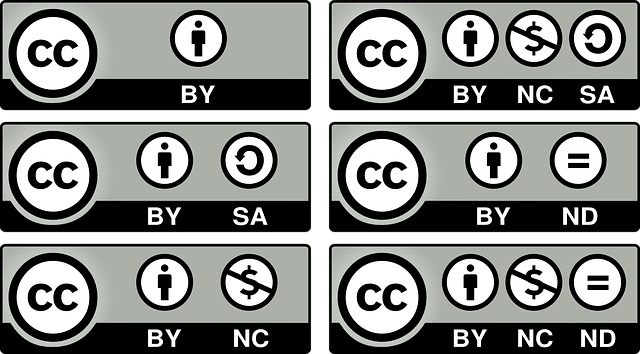
\includegraphics[width=0.5\textwidth]{assets/creative-commons-licenses.png}
	\caption{Le possibili combinazioni per licenze Creative Commons}
\end{figure}



\section{La necessità della piattaforma}
Attualmente le modalità di accesso e di approvazione per le risorse pubblicate
da SapienzaNLP sono molteplici e diverse tra loro: per alcune è
necessario effettuare una richiesta tramite email, per altre è disponibile il download
diretto tramite la repository su GitHub, ma è anche possibile che sia necessario
registrarsi con i propri dati sulla pagina web relativa alla risorsa e successivamente
attendere che venga approvata la richiesta.
La frammentarietà di questo approccio consente di evidenziare in particolare tre problemi:
\begin{itemize}
	\item non tutte le modalità di accesso verificano che l'utente approvi esplicitamente
	le licenze d'uso con cui vengono fornite le risorse
	\item l'utente può trovarsi a dover gestire più credenziali d'accesso (username
	e password) per le pagine web da cui scaricare le relative risorse
	\item la gestione e l'approvazione degli accessi risulta essere complessa
\end{itemize}

Lo scopo è quindi quello di avere un unico portale per richiedere l'accesso alle
risorse, gestire lo stato di approvazione delle richieste e far approvare
esplicitamente le modalità con cui è concesso l'utilizzo dei dati.

La piattaforma sviluppata rende possibile visualizzare tutte le risorse
disponibili per il download e selezionarne una o più per richiederne l'accesso.
Fornisce inoltre un modulo pdf, generato dinamicamente, contenente le clausole
specifiche da dover firmare per poter effettuare la richiesta. La possibilità di
effettuare il download può essere poi concessa da un amministratore, che revisiona
i dati dell'utente e il modulo di richiesta, e può garantire l'accesso alle risorse
richieste (o a parte di esse) generando dei link di download utilizzabili
solamente dall'utente richiedente.

% !TeX root = ../relazione.tex

\chapter{Analisi dei requisiti}


\section{Requisiti piattaforma}
Gli attori\footnote{Coloro che interagiscono con il sistema} del sistema
sono suddivisi nelle seguenti tipologie:
\begin{itemize}
	\item \textbf{Utente web}: usufruisce delle risorse di SapienzaNLP e utilizza
	la piattaforma per richiederne l'accesso o per scaricarle
	\item \textbf{Utente gestore}: gestisce le richieste effettuate, ne
	può cambiare lo stato (ad esempio approvandole o rifiutandole) e può generare
	dei link di download tramite cui scaricare le risorse associate
\end{itemize}

\paragraph{Selezione delle risorse}
Gli utenti web possono selezionare una o più risorse per cui richiedere l'accesso,
aggiungendo una descrizione dell'utilizzo che se ne vuole fare. A questa azione
segue la generazione di un pdf contenente un resoconto e le informazioni legali
che l'utente dovrà approvare per poter richiedere l'accesso alle risorse richieste.

\paragraph{Richiesta di accesso} \label{par:access-request}
Gli utenti web possono sottomettere una richiesta di accesso alle risorse, inserendo
i propri dati e il pdf precedentemente generato, firmato dove richiesto.
I dati richiesti all'utente sono i seguenti: nome, cognome, username, email,
azienda/organizzazione e paese di provenienza.

\paragraph{Autenticazione amministrazione}
Gli utenti gestori, possono accedere ad un pannello di amministrazione
effettuando l'autenticazione tramite username e password.

\paragraph{Cronologia delle richieste}
Gli utenti gestori, tramite il pannello di amministrazione, possono accedere allo
storico di tutte le richieste di accesso alle risorse effettuate, ordinate
cronologicamente.

\paragraph{Dettaglio e accettazione/rifiuto richiesta}
Gli utenti gestori, tramite il pannello di amministrazione, possono accedere ai
dettagli delle richieste effettuate, visualizzarne il modulo pdf associato e
cambiare lo stato della richiesta, approvandola o rifiutandola.
La cronologia dei cambiamenti di stato, e l'utente che li ha effettuati, viene
mostrata insieme ai dettagli.

\paragraph{Generazione di link per il download}
Gli utenti gestori, tramite il pannello di amministrazione, possono generare dei
link di download per una o più risorse relativamente ad una richiesta di accesso.
Questi link vengono inviati automaticamente all'email dell'utente che ha effettuato
la richiesta, tramite cui potrà scaricare le risorse.



\section{Raffinamento e funzionalità aggiuntive}
I requisiti appena elencati rappresentano le funzionalità essenziali per permettere
accesso e gestione delle risorse, ovvero lo scopo principale della piattaforma.
È però necessario tenere anche conto dei dati relativi ad utenti gestori, alle
risorse e alle loro versioni; è quindi seguita una fase di raffinamento dei
requisiti e delle funzionalità.


\subsection{Utenti}
Viene aggiunta una terza tipologia di utente, l'\textbf{Utente amministratore}
che può accedere al pannello di amministrazione tramite autenticazione e, oltre
alle richieste effettuate, può visualizzare e gestire gli utenti, le risorse e
le relative versioni. Può accedere a tutte le funzionalità della piattaforma.
Le tipologie di presenti nella piattaforma sono quindi le seguenti:
\begin{itemize}
	\item Utente web
	\item Utente gestore
	\item Utente amministratore
\end{itemize}


\subsection{Autenticazione}
Per semplificare il processo di inserimento dei dati da parte di un utente web
che richiede l'accesso alle risorse (\ref{par:access-request}) ed evitare che
per ogni ogni nuova richiesta debbano essere re-inseriti gli stessi dati, l'accesso
alla piattaforma viene gestito da una procedura di autenticazione per tutti gli
utenti. In questo modo se uno stesso utente effettua più volte delle richieste,
i dati necessari saranno già presenti nel sistema e sarà necessario aggiungervi
solamente il modulo pdf firmato.

\paragraph{Registrazione}
Viene quindi aggiunta la possibilità di registrarsi alla piattaforma inserendo i
dati che erano previsti per le richieste di accesso alle risorse. Questa procedura
permette di creare un nuovo utente web, che quindi non avrà accesso al pannello
di amministrazione. La registrazione non prevede la scelta di una password, che
viene invece generata automaticamente e inviata tramite email all'utente.

\paragraph{Recupero password}
Per tutte le tipologie di utente viene data la possibilità di generare una nuova
password, inviata tramite email, che diventa permanente nel momento in cui
viene utilizzata per effettuare l'accesso.

\paragraph{Autenticazione}
Ad esclusione di \textbf{Registrazione} e \textbf{Recupero password}, per utilizzare
le funzionalità della piattaforma relative alla propria tipologia di utente,
deve essere prima effettuata l'autenticazione inserendo username e password.


\subsection{Gestione utenti}
Le funzionalità descritte in questa sezione sono riservate ai soli utenti
amministratori.

\paragraph{Lista utenti esistenti}
È possibile visualizzare una lista di tutti gli utenti registrati nella piattaforma
e avere un resoconto delle relative informazioni principali.

\paragraph{Dettaglio utente esistente}
È possibile visualizzare e modificare i dati degli utenti, ad eccezione della
password, e visualizzare uno storico:
\begin{itemize}
	\item delle richieste effettuate, se utente web
	\item dei cambi di stato delle richieste, se utente gestore o amministratore
\end{itemize}

\paragraph{Disabilitazione utente esistente}
È possibile disabilitare un utente, negandogli la possibilità di autenticarsi e,
di conseguenza, di utilizzare qualunque funzionalità della piattaforma.
Questa azione non elimina l'utente ed è reversibile, viene mantenuto lo storico
delle richieste e dei cambi di stato effettuati.

\paragraph{Creazione utente gestore}
È possibile creare un nuovo utente gestore, abilitato ad accedere al pannello
di amministrazione. Come per la registrazione di un utente web, la password viene
generata automaticamente e inviata all'email specificata.


\subsection{Gestione risorse}
Le funzionalità descritte in questa sezione sono riservate ai soli utenti
amministratori.

\paragraph{Lista risorse esistenti}
È possibile visualizzare una lista di tutte le risorse disponibili nella
piattaforma e avere un resoconto delle relative informazioni principali.

\paragraph{Dettaglio risorsa esistente}
È possibile visualizzare e modificare i dati delle risorse e visualizzare le
versioni associate.

\paragraph{Eliminazione risorsa esistente}
È possibile eliminare definitivamente dalla piattaforma una risorsa e tutte le
versioni associate.

\paragraph{Creazione nuova risorsa}
È possibile aggiungere una nuova risorsa, specificando un nome, una descrizione
e la licenza con cui viene fornita.

\paragraph{Creazione e modifica versione risorsa}
È possibile aggiungere e modificare una versione di una risorsa, specificandone
il nome, la data di rilascio e il file a cui fa riferimento per il download.

% !TeX root = ../relazione.tex

\chapter{Progettazione}


\section{Architettura} \label{sec:architettura}
Il progetto è basato su una architettura 3-tier \cite{wiki:3-tier-architecture},
ovvero è suddiviso in 3 diversi moduli sviluppati separatamente e dedicati alla
gestione dei dati (\textbf{Data tier}), alla logica funzionale (Logic o
\textbf{Application tier}) e all'interfaccia utente (\textbf{Presentation tier});
questi comunicano e scambiano dati tra loro con un approccio client-server.

\begin{figure}[ht]
	\centering
	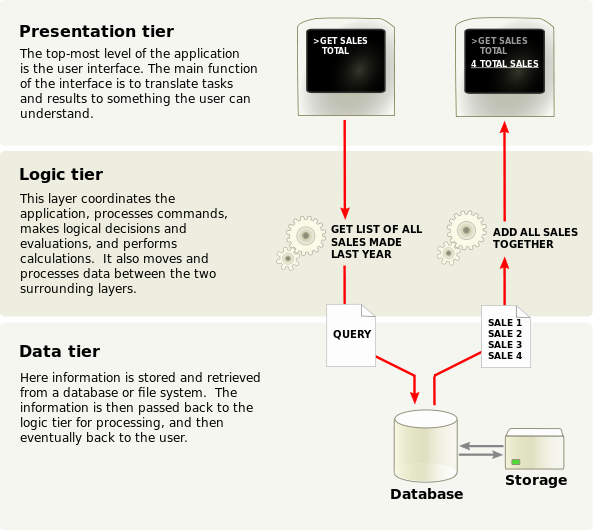
\includegraphics[width=0.6\textwidth]{assets/diagrams/3-tier-architecture.png}
	\caption{Schema architettura web 3-tier}
	\label{fig:3-tier-architecture}
\end{figure}

Con questa architettura è possibile raggiungere un buon livello di scalabilità
e modularità, evitando di includere la logica dell’applicazione sia a livello del
server che lato client (modello 2-tier).
Il terzo livello software inserito nel mezzo contiene la maggior parte della logica
e si posiziona ad un livello intermedio in modo da essere disponibile ad ogni
servizio del sistema. Nel momento in cui è necessario cambiare un componente di
logica dell’applicazione è sufficiente modificare solo un "mattoncino" specifico del
livello intermedio.
Ognuno dei tre livelli architetturali è associato ad un specifica categoria logica:
\begin{itemize}
	\item Il Presentation tier sarà la UI (User Interface) dei servizi per l’utente,
	garantendogli la possibilità di interagire con gli altri livelli tramite
	un'interfaccia grafica, in maniera trasparente
	\item L'Application Tier si occupa della parte applicativa e logica,
	include l’esecuzione di applicazioni, la logica che si occupa della convalida
	dei dati e delle richieste/risposte nella comunicazione fra i processi degli
	altri livelli
	\item Il Data Tier include i servizi che gestiscono il database; che forniscono
	i dati necessari al completamento delle richieste del livello Logico. In questo
	caso la logica del server interagisce con la gestione, l’accesso e la sicurezza
	dei dati
\end{itemize}
Tra i vantaggi di questa architettura possiamo includere la distribuzione e la
riusabilità del codice, in quanto tutte le logiche che vengono utilizzate dagli
utenti finali sono nel server intermedio. Un'altra caratteristica è che questa
separazione tra l'interfaccia utente, la logica ed i dati permette una maggiore
flessibilità nello sviluppo di nuove funzionalità; ad esempio dato che le
componenti server e logiche sono già testate, lo sviluppo di un nuovo componente
nella UI sarà più rapido e con una fase di test più breve. In pratica un
aggiornamento, il fix di un bug o l'implementazione di una nuova funzionalità di
un singolo livello applicativo ha un impatto minimo sugli altri.

L'approccio si riflette anche nella gerarchia delle competenze, in quanto gli
eventuali team di sviluppo si possono separare in diverse tipologie per
specializzarsi negli ambiti relativi ai 3 livelli dell'architettura: il front-end,
il back-end ed il data-end. La scalabilità è un aspetto fondamentale di questa
architettura in quanto separando i diversi livelli ognuno può scalare in termini
di capacità e potenza indipendentemente dagli altri. Per esempio se stiamo ricevendo
un numero elevato di richieste web che non si stanno traducendo in un carico
direttamente proporzionale in richieste computazionali che caricano le applicazioni,
possiamo scalare solo questo livello.

\section{Sessione utente}
Trattandosi di una piattaforma web le cui funzionalità sono pensate per essere
accessibili solo a seguito di autenticazione, la gestione della sessione utente
ne è una parte molto importante. Una sessione rappresenta infatti la possibilità
che un utente possa usufruire di un servizio in maniera continua, senza doversi
autenticare ad ogni operazione che necessita di verificare che si sia in possesso
di un account valido o che si abbiano permessi sufficienti.

\paragraph{Approccio basato su token}
L'approccio utilizzato è quello basato su \textbf{token}, per cui a seguito
di ogni autenticazione deve essere generato e associato all'utente un codice
univoco, volto a verificare la sessione. Questo codice, detto \textit{token}, è
definito come valido per un breve periodo di tempo, ma viene "rinnovato" ad ogni
richiesta effettuata dal client verso l'Application tier, così da garantire la
continuità della sessione, fino alla scadenza o al logout esplicito da parte
dell'utente.
Per ogni richiesta effettuate viene quindi verificato che l'utente sia autenticato
e che sia autorizzato ad effettuare eventuali operazioni riservate (ad esempio
accedere al pannello di amministrazione).


\section{Diagramma ER}

\begin{wrapfigure}{r}{0.4\textwidth}
	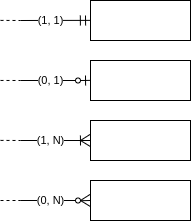
\includegraphics[width=\linewidth]{assets/diagrams/crows-foot-notation.png}
	\cprotect\caption{notazione \textit{crow's foot}}
	\label{fig:crows-foot-notation}
\end{wrapfigure}

Il diagramma in \autoref{fig:er-diagram} è stato progettato con MySQL WorkBench
\cite{workbench:9-EER} ed utilizza la notazione \textit{crow's foot}
\cite{wiki:crows-foot}, più orientata all'implementazione, in cui le relazioni
sono rappresentate da linee che collegano le entità e la cui cardinalità è
espressa tramite i simboli presenti alle estremità (\autoref{fig:crows-foot-notation}).

\begin{figure}[ht]
	\centering
	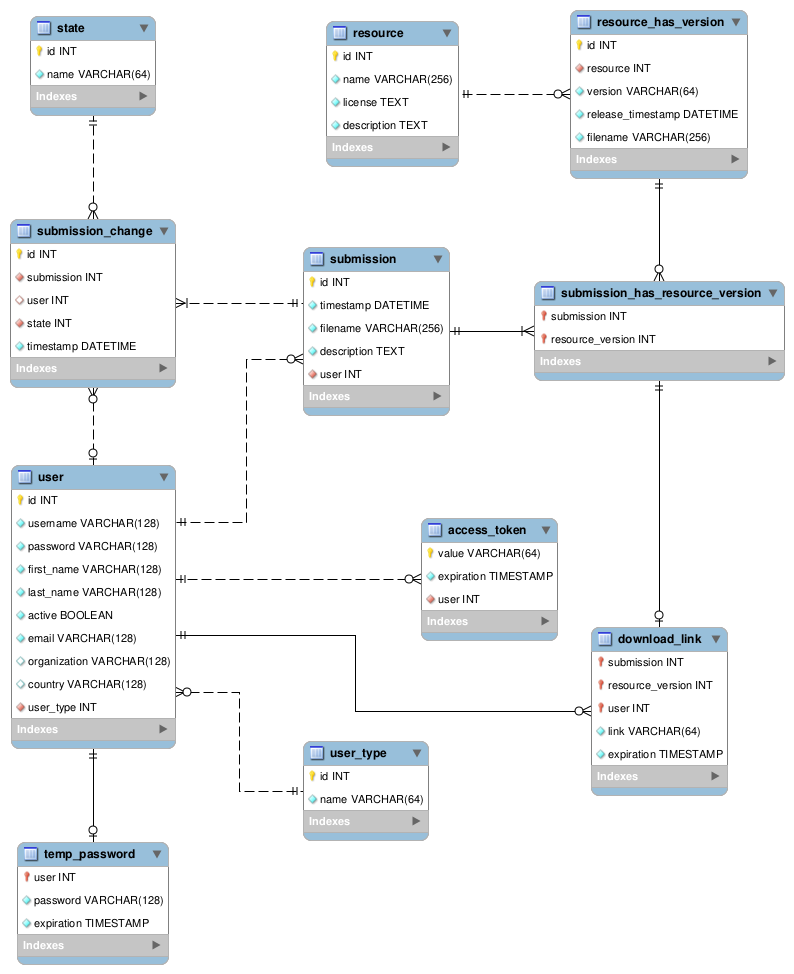
\includegraphics[width=\textwidth]{assets/diagrams/db-er-diagram.png}
	\caption{Diagramma ER}
	\label{fig:er-diagram}
\end{figure}

% !TeX root = ../relazione.tex

\chapter{Implementazione}


\section{Data tier}
Questo modulo comprende il database, per il quale è stato scelto \textbf{MariaDB},
una soluzione open source sviluppata dagli autori di MySQL, e implementa delle
API per poter stabilire facilmente una connessione con esso ed effettuare
modifiche e interrogazioni, mappando le operazioni \textbf{CRUD} (Create, Retrieve,
Update e Delete).

\paragraph{Pattern DAO}
Per l'implementazione si è utilizzato \textbf{Java} come linguaggio di programmazione
e il \textbf{Design Pattern DAO} (Data Access Object). Per ogni entità del database
sono state quindi definite:
\begin{itemize}
	\item Una classe \textbf{DTO} (Data Transfer Object), che rappresenta la
	relativa entità, le cui istanze vengono utilizzate per lo scambio dei dati
	con il database
	\item Un'interfaccia \textbf{DAO} che definisce i metodi che si possono
	utilizzare per interagire con la relativa entità del database, tra cui le
	operazioni CRUD necessarie per assolvere i requisiti del sistema
	\item Almeno una classe che implementi il DAO, responsabile dell'effettiva
	connessione con il database e della logica con cui i metodi accedono ai dati
\end{itemize}

\lstinputlisting[language=Java, caption=Interfaccia DAO relativa all'entità \textit{user}]{assets/code/UserDAO.java}

Questa struttura migliora ulteriormente la modularità e la flessibilità del
progetto (\autoref{sec:architettura}); ad esempio se fosse necessario utilizzare
una diversa tecnologia per il database sarebbe sufficiente una nuova
implementazione del DAO, che ovviamente manterrebbe gli stessi metodi.

\paragraph{Project Lombok}
Una libreria open source che è stata molto utilizzata per ridurre i tempi di
scrittura e migliorare la leggibilità del codice è \textbf{Project Lombok};
un \textit{Annotation processor} che, tramite delle annotazioni nel codice,
sostituisce la scrittura di metodi molto comuni e simili tra loro (come
\textit{setter} o \textit{getter}).
Nelle classi che rappresentano dei dati, come le classi DTO, questo è stato
essenziale per poter scrivere in poche righe un codice chiaro e funzionale;
ad esempio, la classe \texttt{User} (\ref{code:user-dto}), grazie alle annotazioni
\texttt{@Getter}, \texttt{@Builder} e \texttt{@Setter}, dispone di metodi get
per ogni campo, di un'implementazione del pattern Builder e di un metodo set per
il campo \texttt{id}.

\lstinputlisting[language=Java, label={code:user-dto}, caption=Classe DTO relativa all'entità \textit{user}]{assets/code/UserDTO.java}



\section{Application tier}
In questo modulo viene gestita la parte logica ed applicativa della piattaforma,
tra cui il controllo della sessione utente e i vincoli derivanti dai requisiti;
come ad esempio la possibilità di accedere ad alcune funzionalità solo per certe
tipologie di utenti o il controllo per cui i link di download siano validi solo
per le richieste approvate e solo per l'utente che ha effettuato la richiesta. 


\subsection{Il framework Spring}
Il linguaggio utilizzato è sempre \textbf{Java} ma accoppiato a \textbf{Spring},
un framework per lo sviluppo di applicazioni web, nello specifico nella versione
\textbf{Boot} \cite{spring:boot}, che ne semplifica la configurazione e garantisce
la possibilità di avere un web server \textit{stand-alone} direttamente eseguendo
la classe principale del progetto o effettuandone la build, che produrrà un file
JAR eseguibile con la stessa funzionalità.

\paragraph{Services} \label{par:spring-services}
Per la gestione dell'invio delle email, della generazione del modulo pdf e
dell'interazione con il file system per salvatare i moduli inviati e permettere
il download delle risorse, sono state definite delle classi annotate come
\texttt{@Service}, ovvero relative solo a parte della \textit{business logic}
dell'applicazione. I Service vengono poi utilizzati nel resto del progetto
tramite la \textbf{Dependency Injection} di Spring, che si occupa di fornire la
stessa istanza a tutti i componenti che ne richiedono l'utilizzo. La forma di
injection applicata è quella tramite il costruttore della classe 
(\ref{code:constr-inj}) che viene parametrizzato automaticamente dal framework
all'avvio dell'applicazione.

\lstinputlisting[language=Java, label={code:constr-inj}, caption=Esempio di Constructor Injection per \texttt{EmailService}]{assets/code/AuthenticationController.constructor.java}

\paragraph{Controllers}
Tra i componenti principali del framework troviamo le classi Controller, definite
tramite l'annotazione \texttt{@RestController} e adibite ad eseguire le funzionalità
nel rispetto dei vincoli dell'applicazione. I metodi di queste classi vengono
mappati a degli endpoint del web server che permettono la loro invocazione tramite
richieste HTTP, creando così delle API accessibili tramite l'interfaccia utente.

Ad esempio nella classe \texttt{AuthenticationController} è stato implementato un
metodo \texttt{signUp} (\ref{code:auth-controller-signup}) che permette di
effettuare la registrazione di un nuovo utente. Questo metodo, tramite
l'annotazione \texttt{@PostMapping}, è accessibile effettuando una richiesta POST
all'endpoint \textit{/signup}.

Nel dettaglio, effettua dei controlli sulla validità dei parametri e sull'unicità
di username e indirizzo email, per poi istanziare un nuovo oggetto \texttt{User},
inviare un'email di conferma tramite il Service (\autoref{par:spring-services})
che gestisce le email, inserire l'utente nel database tramite un oggetto DAO e
infine associare un nuovo \texttt{AccessToken} all'utente per garantirgli la sessione.

\lstinputlisting[language=Java, label={code:auth-controller-signup}, caption=Metodo \texttt{signUp} della classe \texttt{AuthenticationController}]{assets/code/AuthenticationController.signup.java}

\paragraph{Filters}
La validità delle sessioni utente e l'accesso alle funzionalità riservate per
utenti amministratori o gestori, sono state gestite tramite dei pattern negli
endpoint; utilizzando ad esempio \textit{/api/admin} come prefisso per tutti
quelli su cui era necessario verificare che l'utente fosse un amministratore
(\ref{code:admin-filter}).

Definendo delle classi che estendono \texttt{OncePerRequestFilter} è stato
possibile implementare dei controlli eseguiti prima di ogni richiesta che rispetti
il pattern specificato, ritornando un codice di errore nel caso le condizioni
non vengano soddisfatte o permettendo l'esecuzione della richiesta altrimenti.

\lstinputlisting[language=Java, label={code:admin-filter}, caption=Filtro per verificare che l'utente possa accedere ad un endpoint riservato]{assets/code/AdminFilter.java}



\section{Presentation tier}

In questo modulo è stata implementata la \textbf{UI} (User Interface), ovvero il
mezzo di comunicazione tra l'utente finale e i moduli precedenti. In questo caso
si tratta di pagine web che presentano le informazioni e guidano l'utente nell'utilizzo
delle funzionalità della piattaforma; che equivalgono a delle richieste HTTP
inviate all'Application tier e a delle conseguenti risposte di conferma o di errore.

\paragraph{Approccio component based}
Per lo sviluppo si è scelta una logica basata su componenti applicata al
paradigma object-oriented, implementata utilizzando \textbf{TypeScript} e JQuery.
TypeScript è un linguaggio di programmazione che estende la sintassi di JavaScript
aggiungendo una forte tipizzazione, le interfacce e altre utili caratteristiche;
mentre JQuery è una libreria utilizzata principalmente per semplificare la
creazione e la manipolazione degli elementi HTML e l'utilizzo di AJAX per
effettuare le richieste.

In questo modulo è stata quindi definita una classe astratta \texttt{AbstractWidget}
per rappresentare i comportamenti comuni di ogni componente della UI. Per ogni elemento
dell'interfaccia che avrebbe dovuto gestire della logica o delle richieste HTTP,
come ad esempio un form per inserire dei dati, è stata implementata una sotto-classe
specializzata a cui è delegata anche la generazione della relativa struttura HTML.

Per quanto riguarda lo stile delle pagine è stato utilizzato Bootstrap per alcune
classi CSS e per il grid-layout, così da garantire un design responsive. Inoltre,
ad ogni Widget è stato associato un file SASS, ovvero un'estensione del classico
CSS, per definire gli stili più specifici.


\subsection{Autenticazione e registrazione}
Le schermate e i widget per l'autenticazione e la registrazione implementano un
form e la relativa richiesta AJAX. La struttura dei due widget è condivisa, di
modo che il bottone per passare da una vista all'altra sia sempre la label sulla
sinistra, mentre sulla destra ci sia sempre quello per effettuare l'azione.

Una volta autenticati, si viene reindirizzati alla successiva schermata in base
alla tipologia di utente, così che un utente web possa direttamente selezionare
le risorse per cui richiedere accesso (v. \autoref{subsec:resources-selection}),
mentre un utente gestore o amministratore possa avere da subito una panoramica
sulle richieste (v. \autoref{subsec:submissions-list}).

\begin{figure}[H]
	\centering
	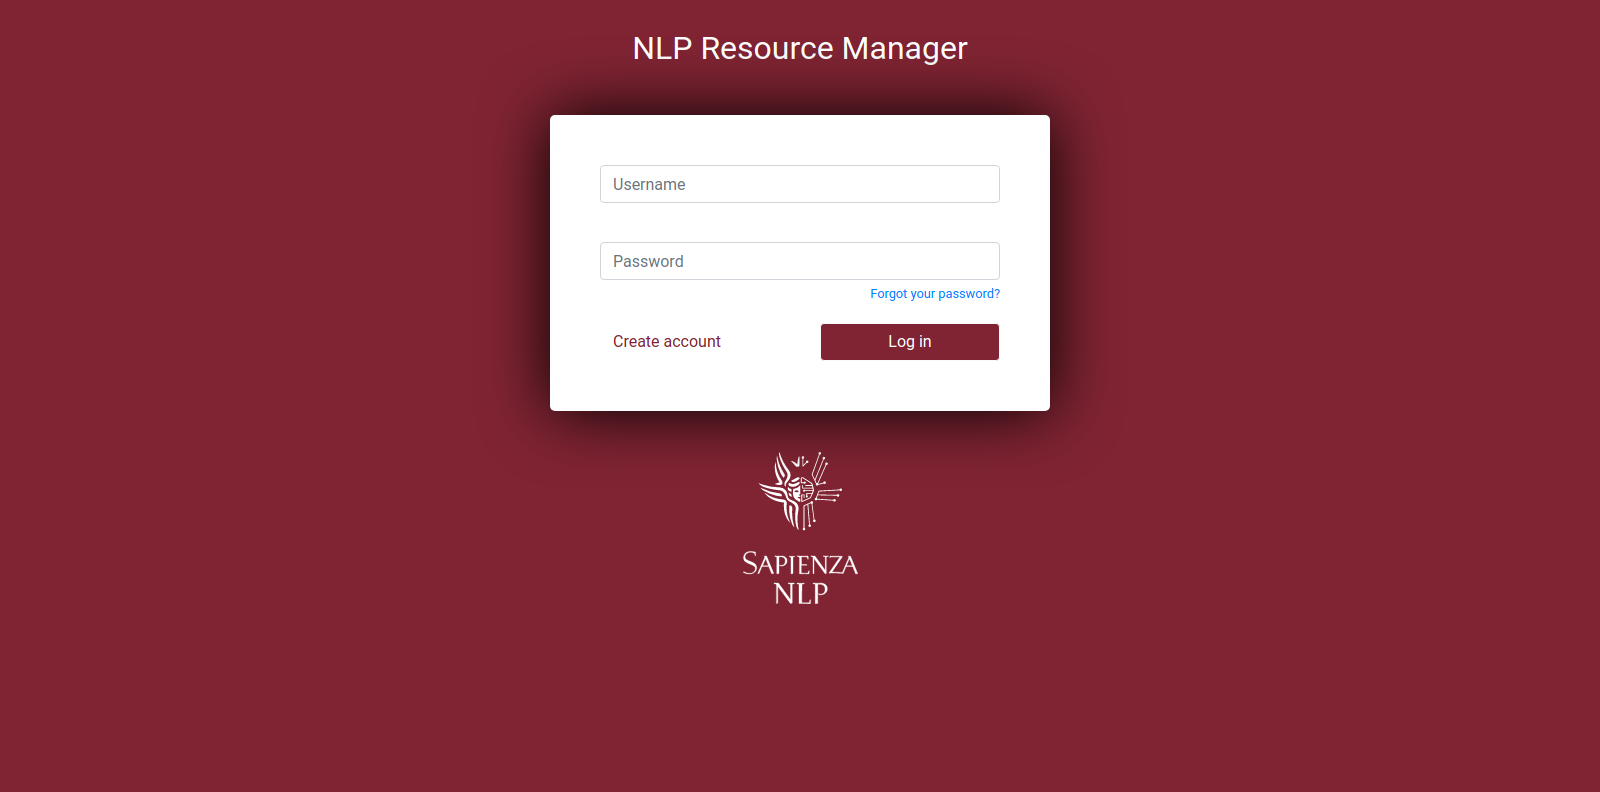
\includegraphics[width=\textwidth]{assets/ui/login.png}
	\caption{Autenticazione}
	\label{fig:login}
\end{figure}

\begin{figure}[H]
	\centering
	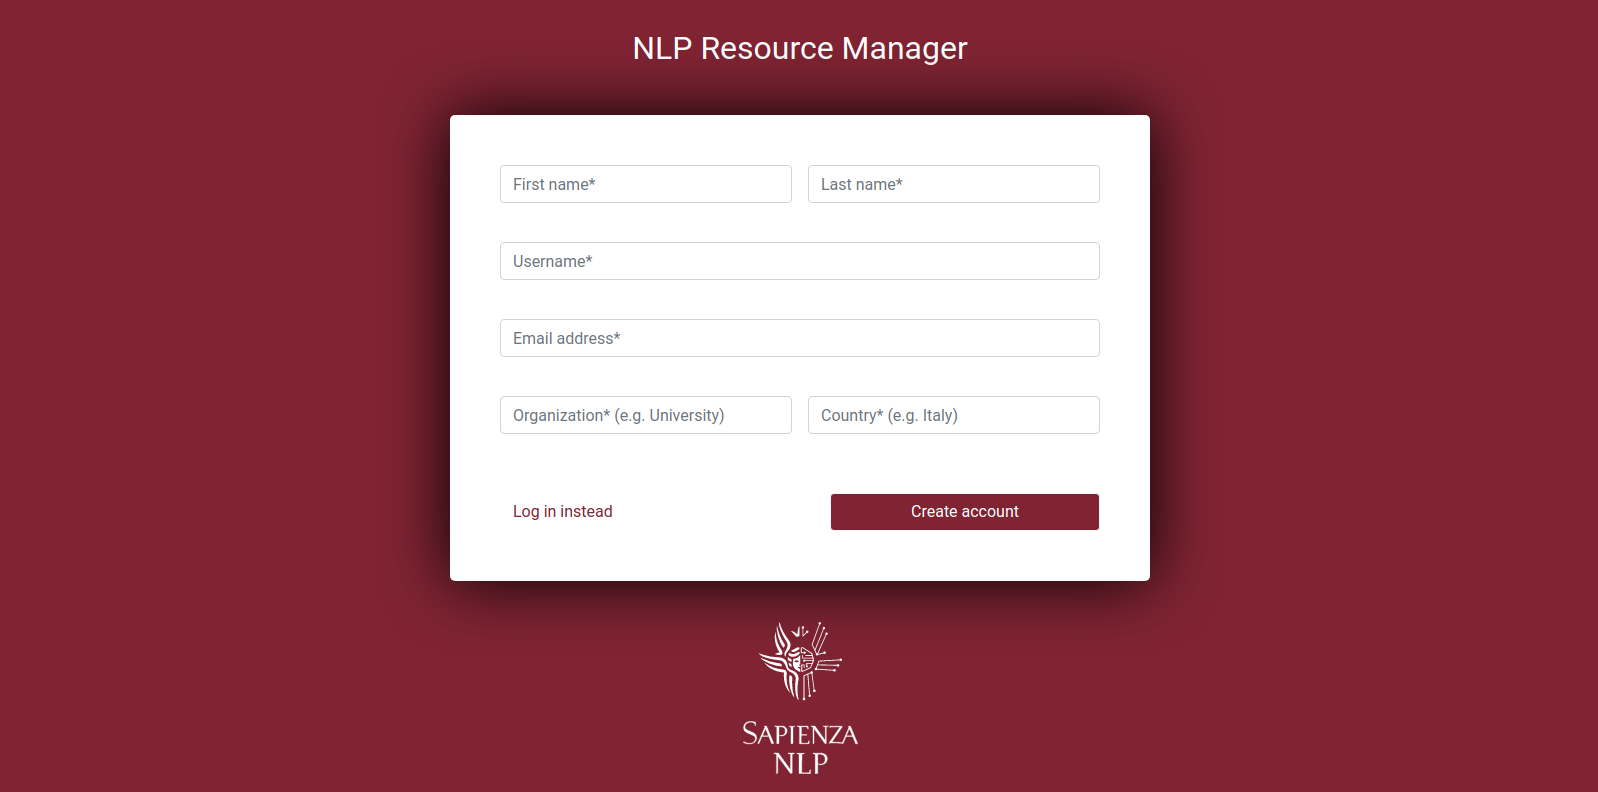
\includegraphics[width=\textwidth]{assets/ui/signup.png}
	\caption{Registrazione}
	\label{fig:signup}
\end{figure}


\subsection{Selezione delle risorse} \label{subsec:resources-selection}
Come in tutte le altre schermate della home, l'interfaccia è divisa in due parti,
con sulla sinistra una sidebar placeholder con i riferimenti Sapienza e sulla
destra il widget principale. In questa schermata il widget si occupa di richiedere
e mostrare la lista di tutte le risorse disponibili, oltre che di gestirne la
selezione multipla e il filtro per parola chiave tramite la barra di ricerca.
L'inserimento della descrizione relativa all'utilizzo previsto è gestito dallo
stesso, con una transizione delle informazioni mostrate e dei bottoni disponibili.

Una volta confermata l'operazione, viene effetuata una richiesta che, in caso di
conferma, ritorna il modulo pdf da dover firmare, scaricato automaticamente dal
client. L'upload del pdf firmato sarà poi possibile dalla schermata successiva
(v. \autoref{subsec:pdf-upload}), accessibile dal menù di navigazione in alto.

\begin{figure}[H]
	\centering
	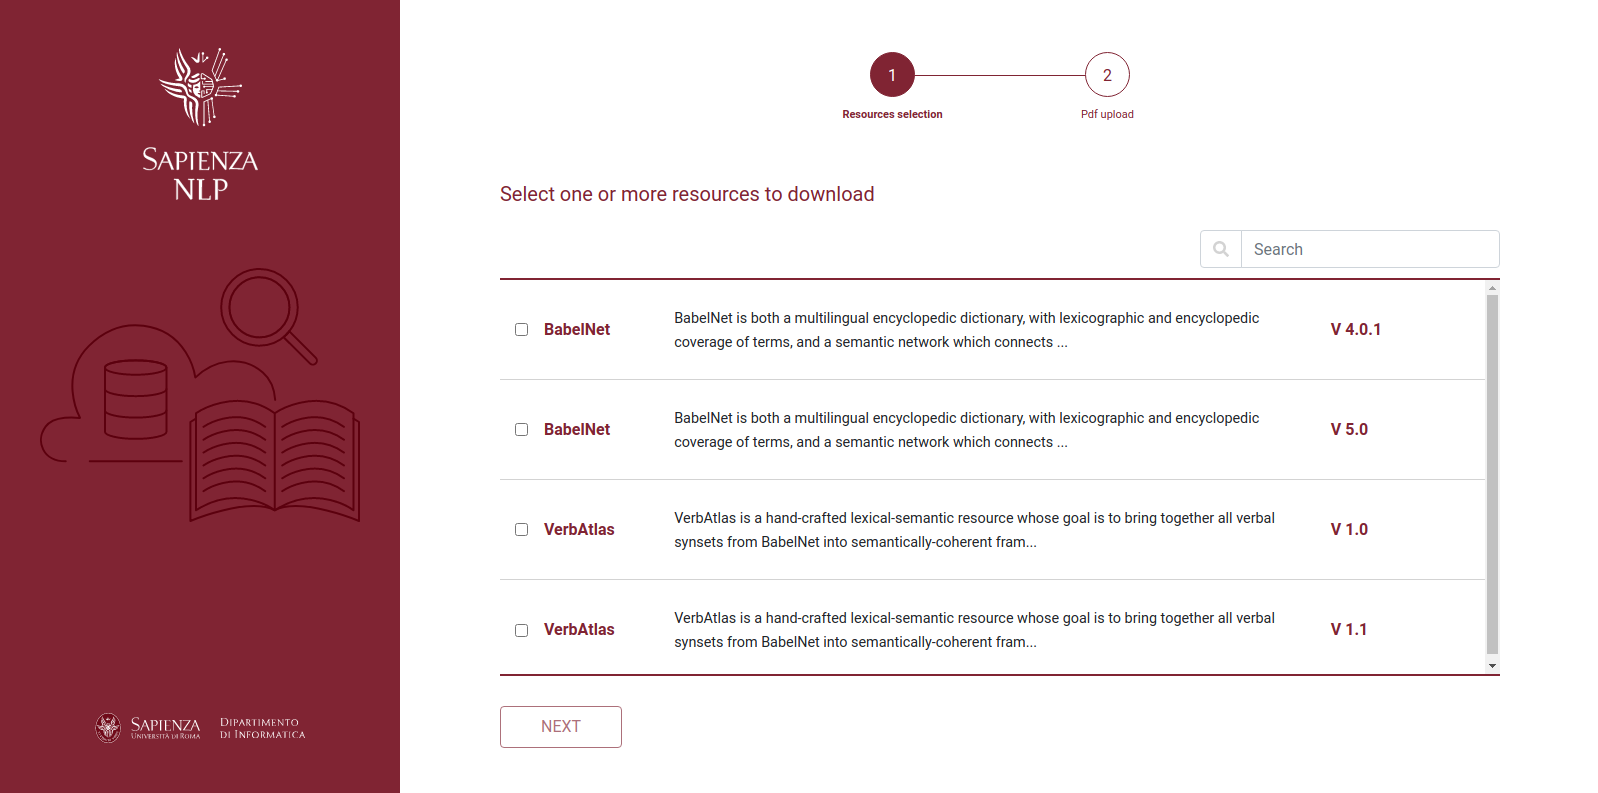
\includegraphics[width=\textwidth]{assets/ui/resources-selection.png}
	\caption{Selezione delle risorse}
	\label{fig:resources-selection}
\end{figure}

\begin{figure}[H]
	\centering
	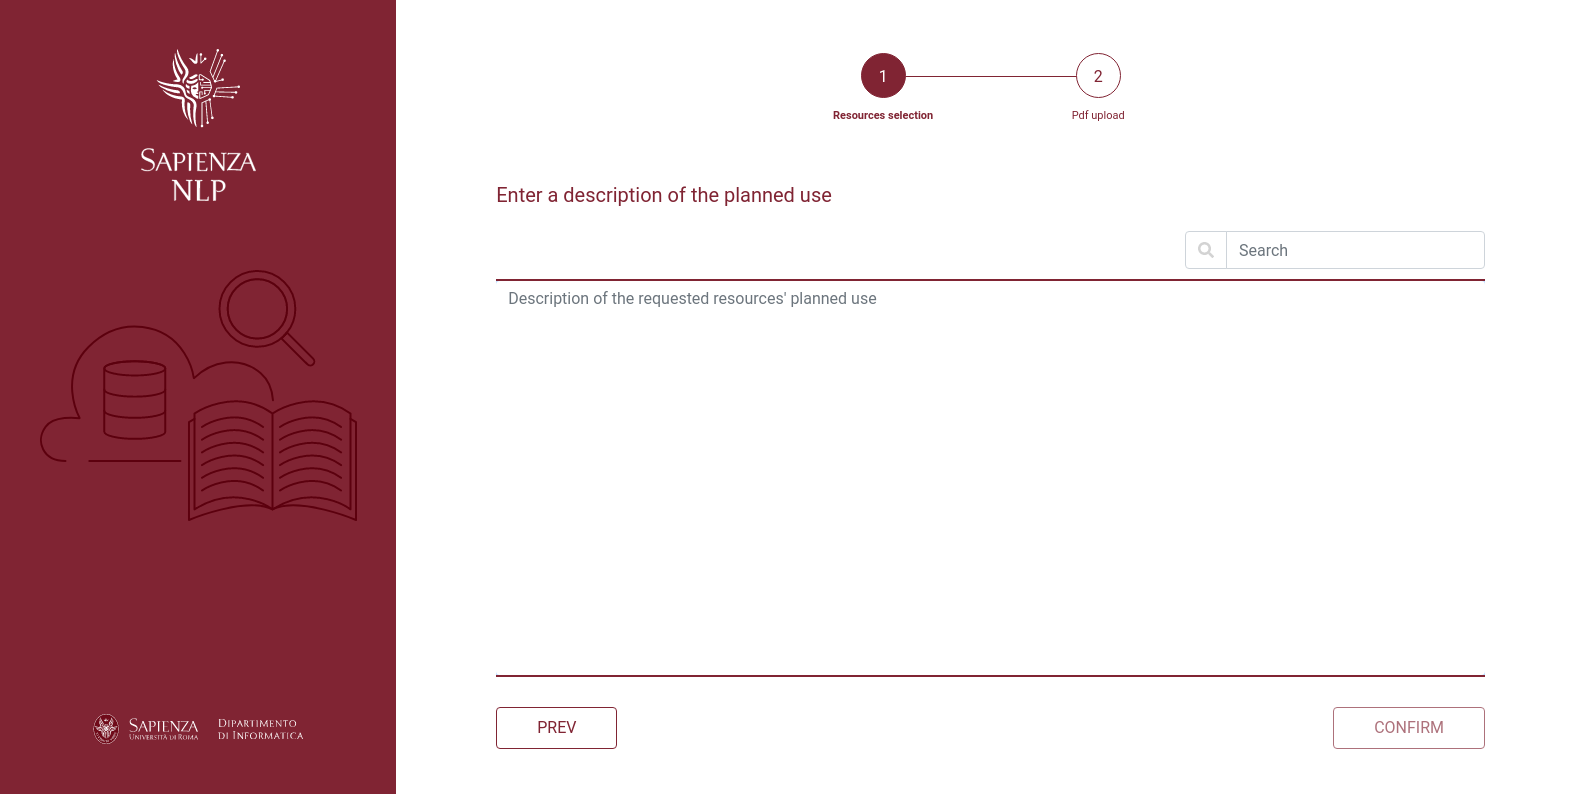
\includegraphics[width=\textwidth]{assets/ui/request-description.png}
	\caption{Inserimento descrizione dell'utilizzo}
	\label{fig:request-description}
\end{figure}


\subsection{Upload del modulo pdf firmato} \label{subsec:pdf-upload}
L'ultimo passo per richiedere l'accesso alle risorse è quello di effettuare
l'upload del modulo pdf firmato. Questa operazione è stata implementata con un
widget per gestire anche il drag and drop e i controlli sulla tipologia e sulla
dimensione del file. Una volta effettuato il \textit{submit}, il server si occupa
in ogni caso di controllare che il file sia in un formato valido e che contenga
dei metadati di validazione e, in caso di successo, il client mostra una
schermata di conferma (v. \autoref{fig:request-success}).

\begin{figure}[H]
	\centering
	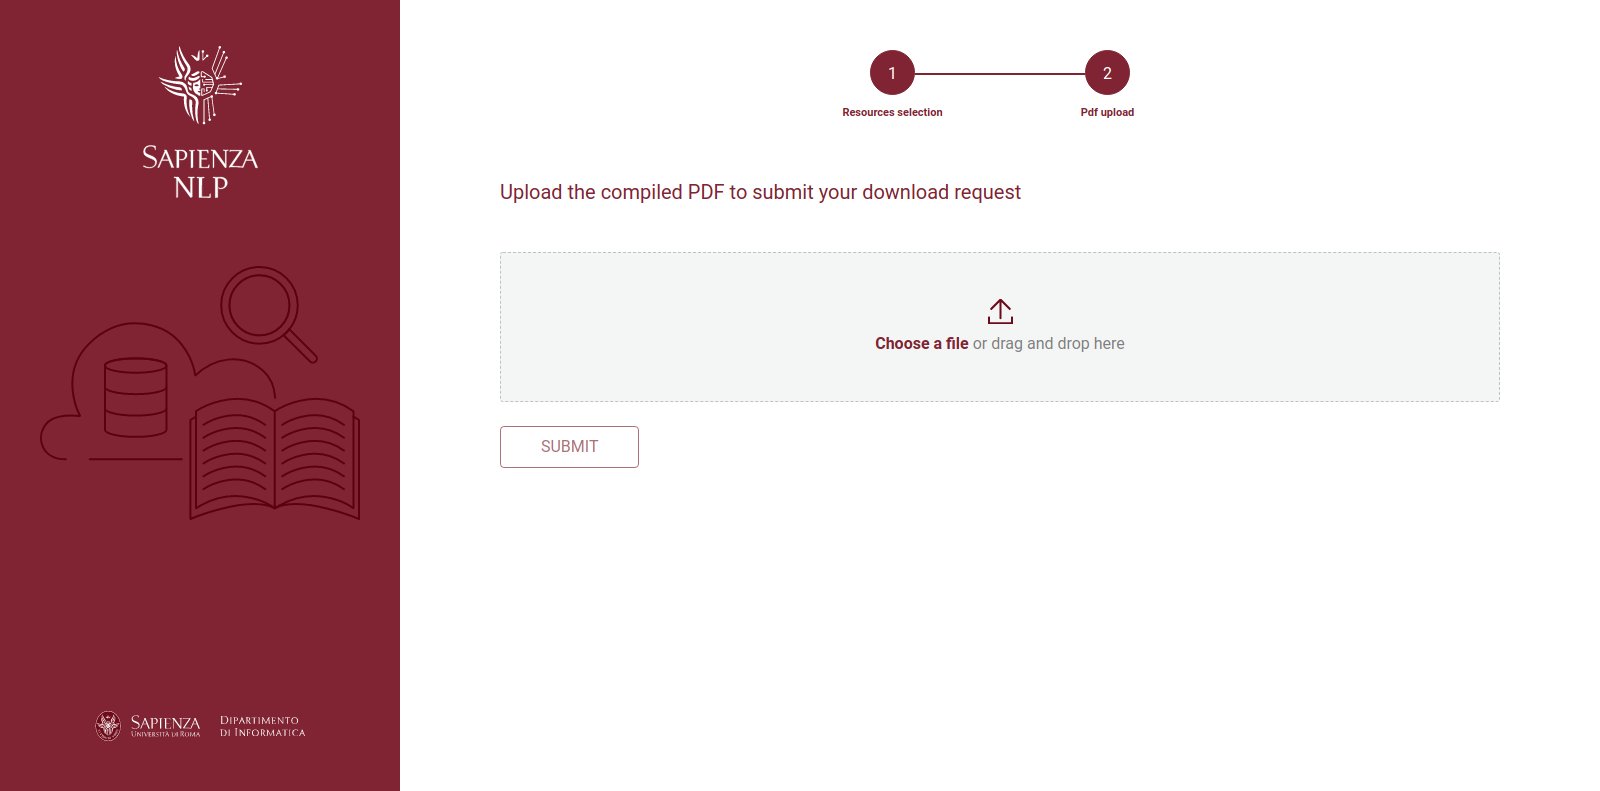
\includegraphics[width=\textwidth]{assets/ui/pdf-upload.png}
	\caption{Upload modulo pdf firmato}
	\label{fig:pdf-upload}
\end{figure}

\begin{figure}[H]
	\centering
	
\includegraphics[width=\textwidth]{assets/ui/request-success.png}
	\caption{Conferma completamento richiesta}
	\label{fig:request-success}
\end{figure}


\subsection{Gestione delle richieste effettuate} \label{subsec:submissions-list}
Nelle schermate di amministrazione l'interfaccia perde la sidebar presente nella
home in favore di una barra di navigazione che permette di accedere alle varie
sezioni del pannello. L'accesso è limitato a soli utenti autorizzati e in caso
il server notifichi una violazione si viene reindirizzati alla schermata di
autenticazione. In questo caso sono presenti più widget, ognuno assolve una
diversa funzionalità, per cui è possibile:
\begin{itemize}
	\item Visualizzare tutte le richieste effettuate, con la data di sottomissione
	lo stato attuale e un bottone per aprirne il dettaglio (v. \autoref{fig:submissions-list})
	\item Visualizzare i dettagli della richiesta, con la possibilità di
	modificarne lo stato e di visualizzare il modulo pdf caricato dall'utente (v. \autoref{fig:submission-details})
	\item Visualizzare lo storico dei cambiamenti di stato, con il relativo utente
	che ha effettuato l'operazione (v. \autoref{fig:submission-details})
	\item Visualizzare la lista delle risorse associate alla richiesta, con la
	possibilità di selezionare per quali generare i link di downloadz (v. \autoref{fig:submission-details})
\end{itemize}

\begin{figure}[H]
	\centering
	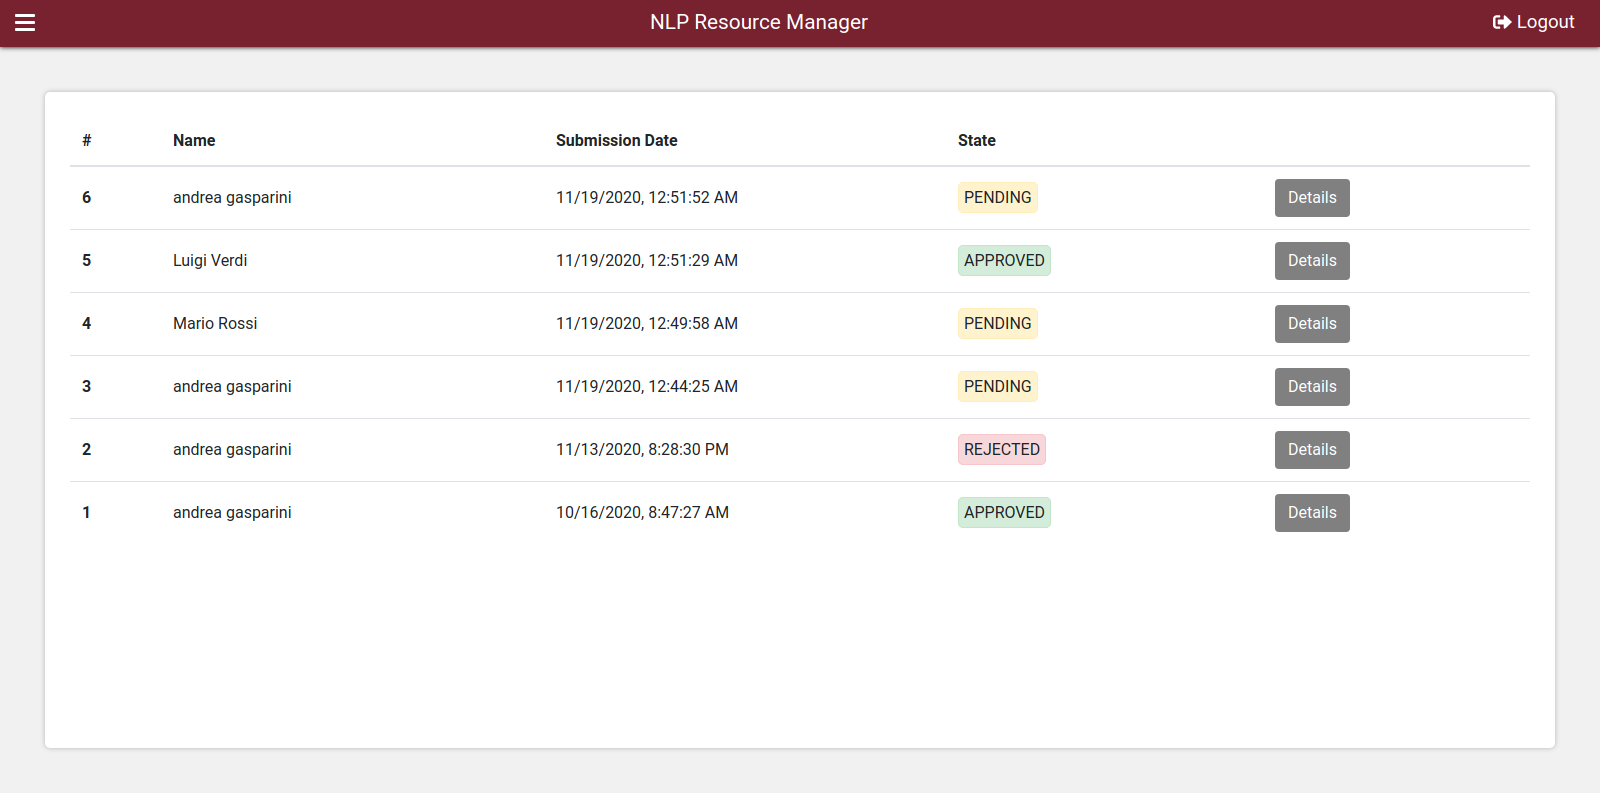
\includegraphics[width=\textwidth]{assets/ui/submissions-list.png}
	\caption{Resoconto di tutte le richieste effettuate}
	\label{fig:submissions-list}
\end{figure}

\begin{figure}[H]
	\centering
	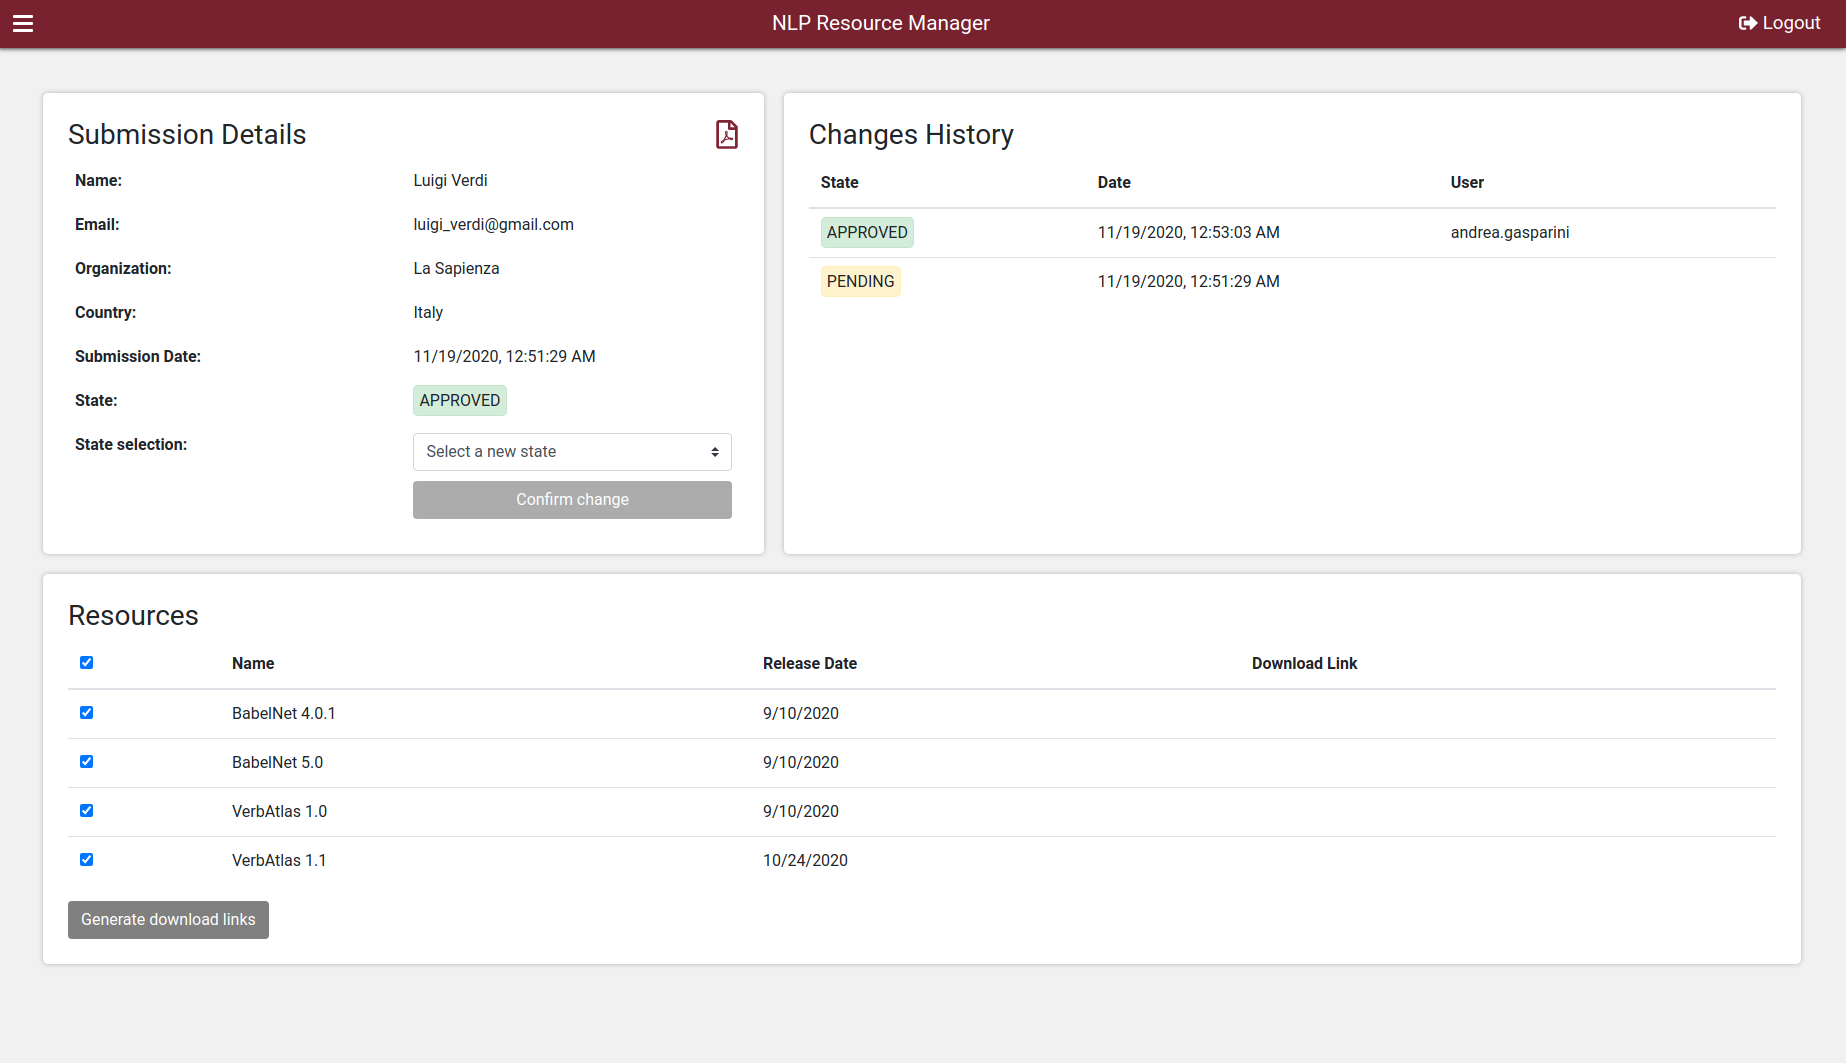
\includegraphics[width=\textwidth]{assets/ui/submission-details.png}
	\caption{Dettaglio di una richiesta effettuata}
	\label{fig:submission-details}
\end{figure}


\subsection{Gestione degli utenti}
In queste schermate di amministrazione è possibile visualizzare un resoconto di
tutti gli utenti registrati e di aprirne un dettaglio, in cui è possibile modificarne
i dati e visualizare la cronologia delle azioni effettuate (richieste sottomesse
o cambi di stato in base alla tipologia di utente). Per il widget relativo alla
cronologia è stato riutilizzato quello già presente nel dettaglio delle richieste
grazie all'approccio modulare basato su componenti che favorisce il riuso del codice.
Allo stesso modo, per creare un nuovo utente viene utilizzando lo stesso widget
che in \autoref{fig:user-details} permette la modifica dei dati di uno già esistente.

\begin{figure}[H]
	\centering
	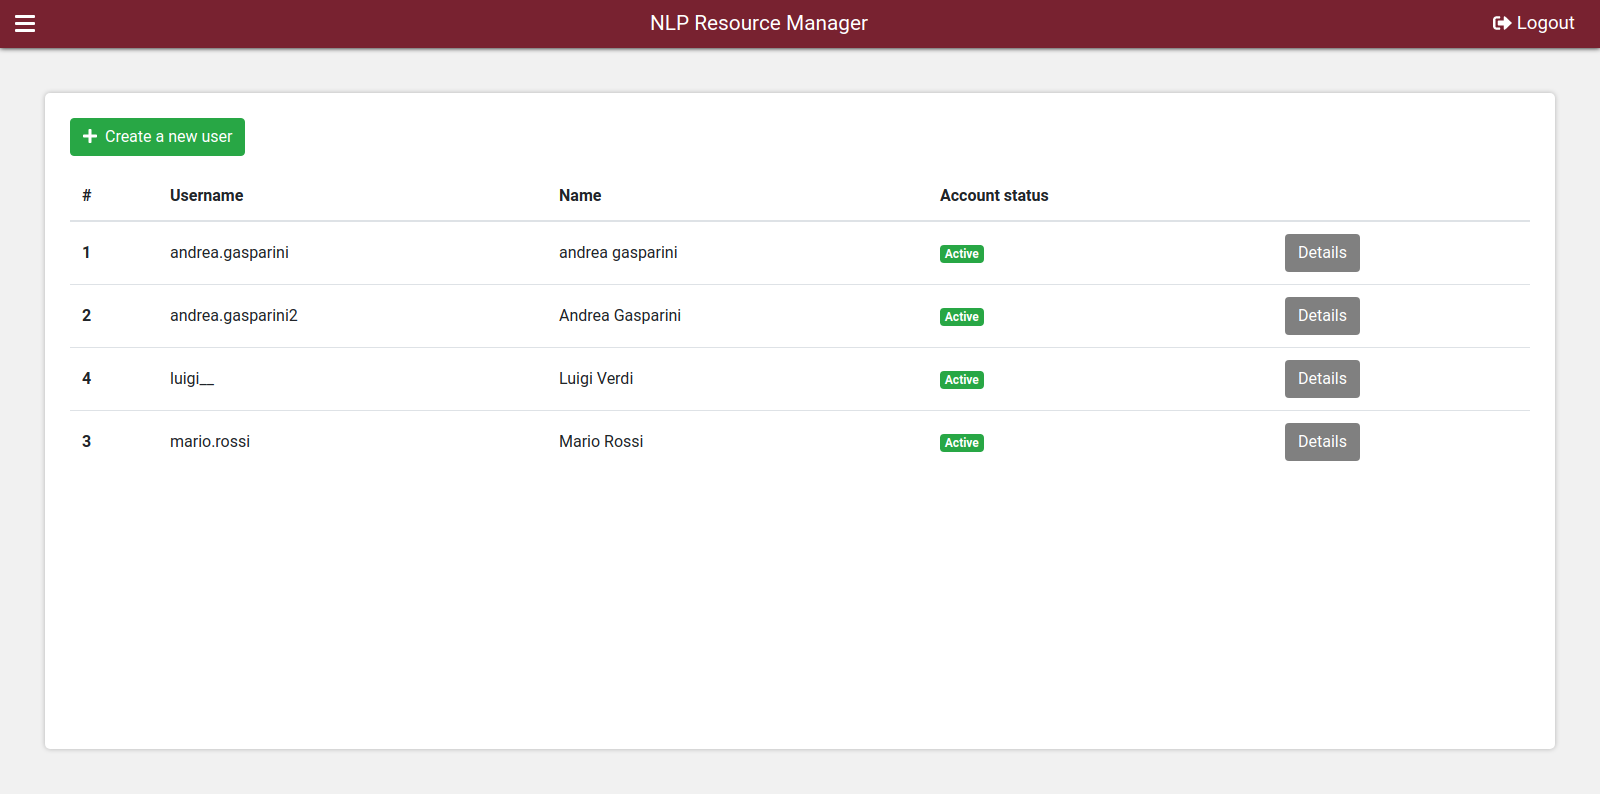
\includegraphics[width=\textwidth]{assets/ui/users-list.png}
	\caption{Resoconto degli utenti registrati}
	\label{fig:users-list}
\end{figure}

\begin{figure}[H]
	\centering
	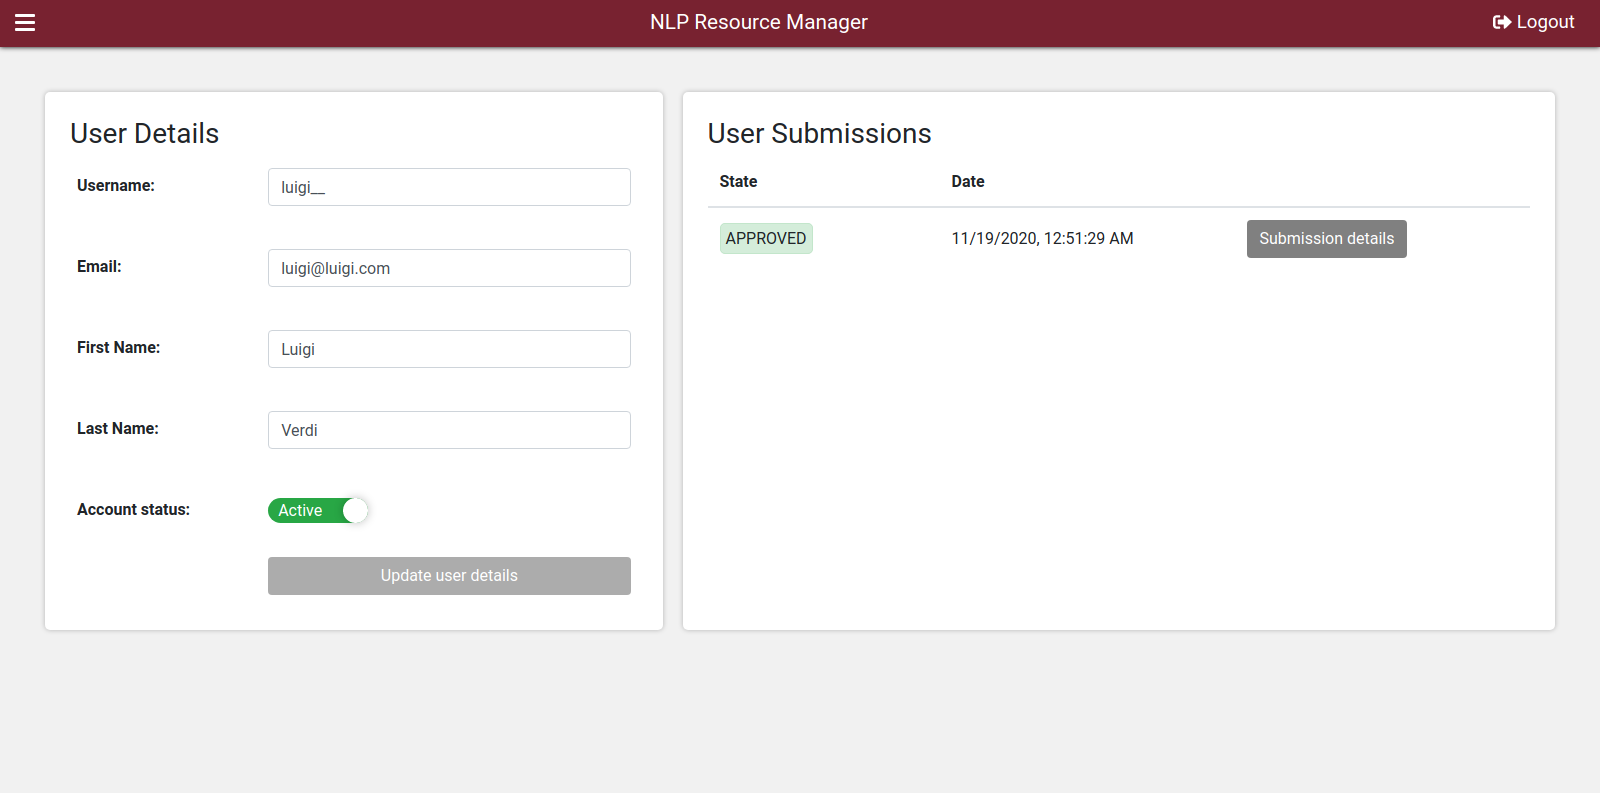
\includegraphics[width=\textwidth]{assets/ui/user-details.png}
	\caption{Dettaglio di un utente}
	\label{fig:user-details}
\end{figure}


\subsection{Gestione delle risorse}
In queste schermate è stata implementata la gestione dell'elemento cardine della
piattaforma, ovvero le risorse. Nel resoconto generale vengono mostrate le risorse
registrate nel database con nome e descrizione, oltre alla possibilità di crearne
di nuove. La selezione di una di esse permette di accedere al dettaglio, in cui
è possibile modificarne i dati, eliminarla definitivamente e aggiungervi una nuova
versione o modificare quelle disponibili.

\begin{figure}[H]
	\centering
	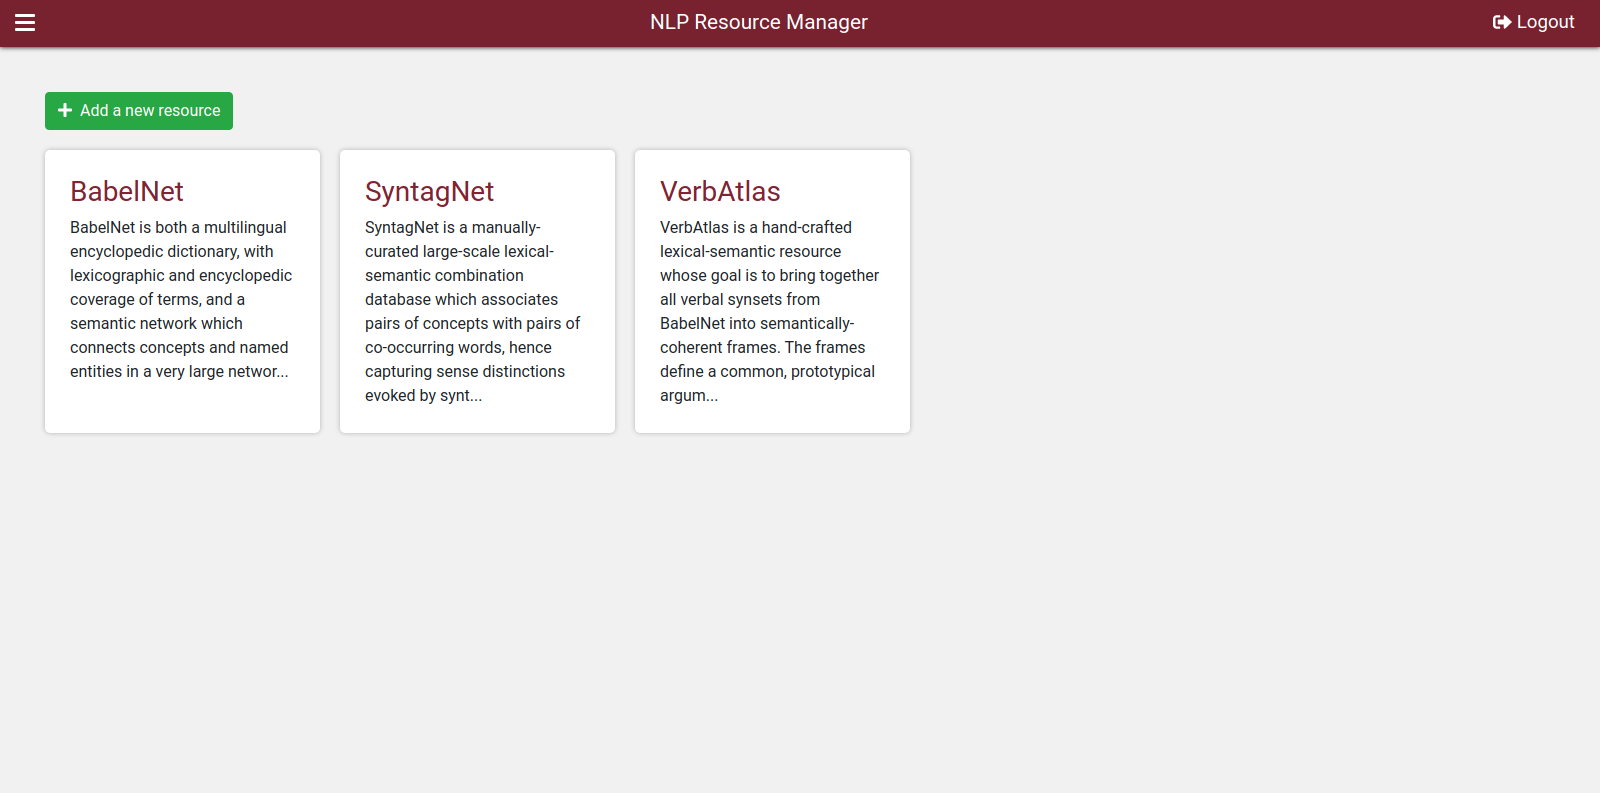
\includegraphics[width=\textwidth]{assets/ui/resources-list.png}
	\caption{Resoconto delle risorse disponibili}
	\label{fig:resources-list}
\end{figure}

\begin{figure}[H]
	\centering
	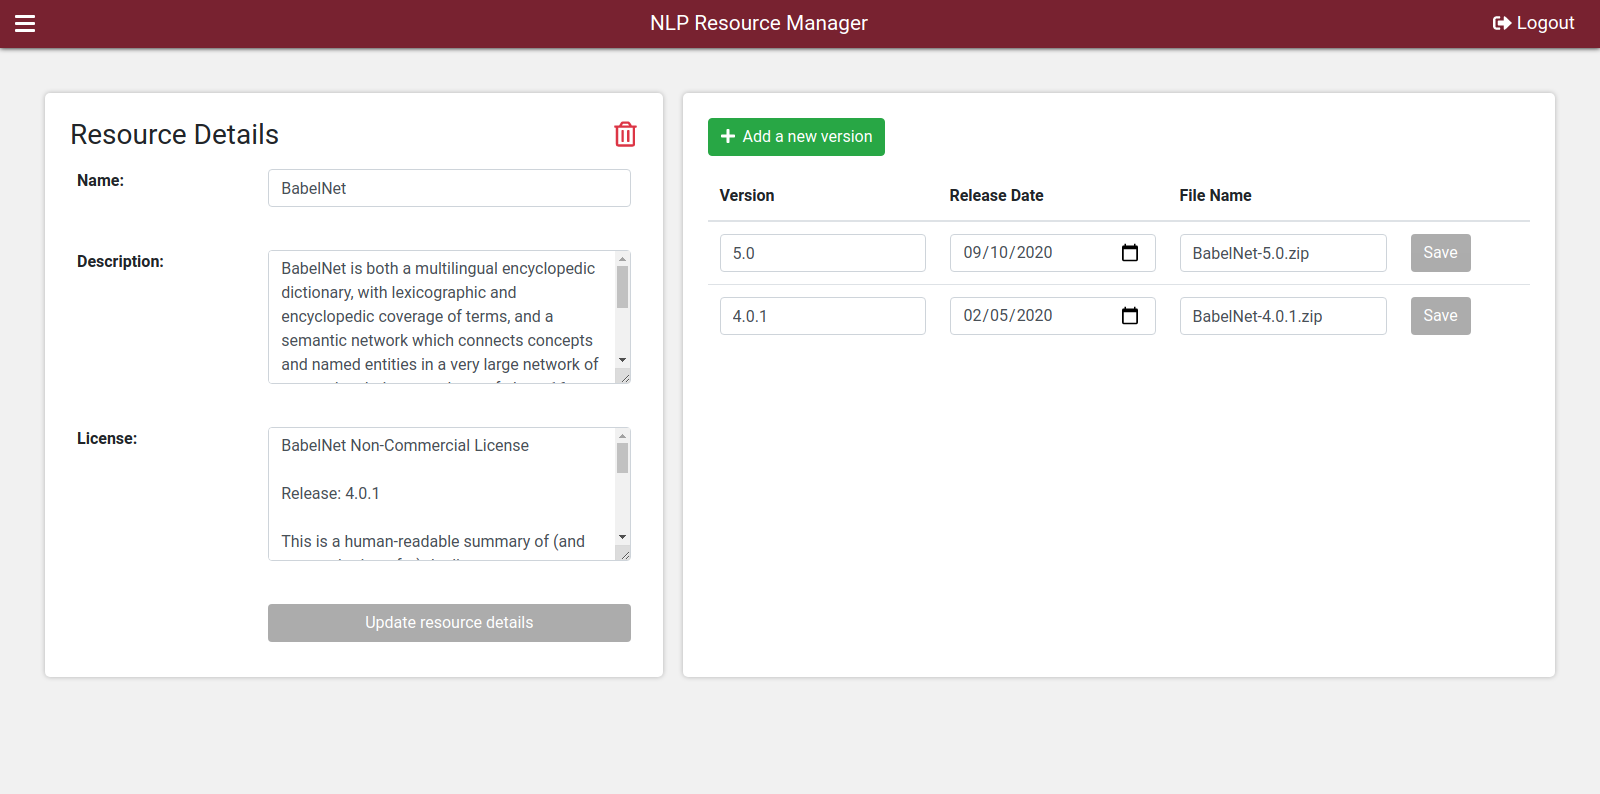
\includegraphics[width=\textwidth]{assets/ui/resource-details.png}
	\caption{Dettaglio di una risorsa}
	\label{fig:resource-details}
\end{figure}

\chapter{Conclusioni}


In questa relazione è stato descritto il lavoro svolto durante l'attività di
tirocinio, inizialmente presentando la necessità di una piattaforma web che permetta
di raccogliere e rendere disponibili in un unico canale le risorse linguistiche
di SapienzaNLP, per poi ripercorrere le principali fasi e scelte affrontate.

Prima dello sviluppo di questo tirocinio era possibile che le modalità di accesso
alle risorse fossero molto diverse diverse tra loro e questo comportava ovviamente
delle difficoltà anche da un punto di vista di gestione. L'utilizzo di queste
è inoltre sempre vincolato dal rispetto delle relative licenze, che solitamente
venivano semplicemente fornite allegate alla risorse scaricate.

Tra gli aspetti che sono stati migliorati troviamo quindi la possibilità di accedere,
tramite un'unica coppia di username e password, a tutte le risorse pubblicate.
La stessa piattaforma e la stessa modalità di autenticazione include inoltre
anche la parte di gestione di quelle disponibili e di approvazione delle
richieste effetuate dagli utenti. In questo modo è stata eliminata la dispersività
che era presente in entrambi i casi ed è stato possibile definire delle modalità
di accesso condivise per tutte le risorse, così da garantire anche una maggiore
flessibilità in caso di eventuale necessità di modifiche.

Un altro miglioramento rispetto alla precedente organizzazione è relativo alla
generazione dinamica di un modulo pdf per la richiesta di accesso alle risorse.
Da un punto di vista di fruibilità si ha il vantaggio di avere i dati dell'utente
inseriti automaticamente, a differenza del classico approccio in cui il modulo è
anonimo e richiede la compilazione nonostante il sistema che lo fornisce conosca
già i dati necessari.
Il modulo risolve inoltre la gestione delle licenze, in quanto quelle relative
alle risorse richieste saranno incluse nel pdf, con relativa clausola specifica
per approvarle esplicitamente firmando.

L'aver realizzato la piattaforma con un approccio modulare ed estendibile è
infine da considerare come il principale vantaggio. È stata infatti ridotta al
minimo la dipendenza tra i vari livelli dell'architettura, così da rendere
possibile facilmente future modifiche e nuove implementazioni. Il fatto che i dati
vengano messi a disposizione tramite chiamate API lascia massima libertà sulla
scelta delle tecnologie per lo sviluppo dell'interfaccia utente, consentendo ad
esempio la creazione di un'equivalente applicazione mobile con le stesse
funzionalità della versione web.
Allo stesso modo la scelta di una nuova tecnologia per il database o per la gestione
della logica applicativa comporterà sempre la sola implementazione del nuovo
modulo.

\paragraph{}
Durante il tirocinio ho avuto modo di applicare alcuni dei concetti appresi nei
vari corsi di studio, dalla gestione delle varie fasi di progettazione
all'applicazione di buone tecniche e paradigmi di programmazione. Mi ha dato
inoltre l’opportunità di imparare e approfondire alcune tecnologie e approcci,
migliorando la mia conoscenza ed esperienza di progettazione e sviluppo per il web.



\section{Sviluppi futuri}
Essendosi conclusa insieme al tirocinio anche la fase più sostanziosa della
realizzazione della piattaforma, è importante valutare a questo punto quelli che
potrebbero essere degli sviluppi futuri per migliorare la qualità e l'utilità del
lavoro svolto.

\paragraph{Integrare un'area personale per gli utenti}
La modalità di accesso alle risorse definita attualmente per la piattaforma prevede
che l'utente riceva tramite email i link per il download, limitando l'utilizzo
dell'interfaccia alla sola fase di richiesta.
Implementando un'area personale, si potrebbe mostrare uno storico delle richieste
effettuate, e grazie ad esso risolvere l'eventualità in cui se ne effettua
più di una per le stesse risorse, ad esempio nel caso in cui non si è più in
possesso dei link di download ricevuti tramite email. Inoltre potrebbe permettere
la modifica dei dati inseriti in fase di registrazione, attualmente possibile solo
tramite il pannello di amministrazione.

\paragraph{Valutare tecnologie alternative}
Essendo stato lo sviluppo e il testing della piattaforma svolto solamente in locale,
in seguito al rilascio ufficiale si potrebbero effettuare delle nuove valutazioni
sulle tecnologie utilizzate e sulle scelte effettuate. Ad esempio sulla tipologia
di database, piuttosto che sul framework per lo sviluppo dell'Application tier.
Ci possono essere molteplici motivi per cui un cambiamento di questo tipo
potrebbe rendersi necessario, ad esempio per un discorso di performance o di
consumi. Importante è quindi aver progettato il sistema per adattarsi facilmente
anche a modifiche che comporterebbero la sostituzione di un intero livello
architetturale (v. \autoref{sec:architettura}).


\backmatter

\cleardoublepage
\phantomsection
\addcontentsline{toc}{chapter}{\bibname}
\bibliographystyle{sapthesis}
\bibliography{references}

\end{document}